\chapter{Design}
\label{cha:design}

Inspired by the success of Transformer architectures on learning sequence modelling tasks in NLP and CV, we propose that we can adapt the same to learn dynamics from network packet data due to the underlying similarity of sequential data. In this chapter, we first present some insights on the data we use for learning, following which, we present the ideas and design choices behind a proposed Transformer architecture which can be used for the same.

\section{Pre-training Dataset}
\label{sec:ns3}
The key requirement for using any deep learning architecture to model and solve a learning problem is the availability good quality training data, which contains enough variation in its  samples in order to capture the underlying distribution effectively. We need enough training data so as the model can learn effectively and not underfit on the training samples. At the same time, we want enough variation in the training data so as to not overfit on a certain subset of features, in order to achieve good generalization benefits from the training process. Given enough data of the right kind, deep learning models are known to exhibit extremely powerful generalizing behaviour\cite{generalizingdnn}.

Acquiring the network packet data to train our proposed NTT model was an initial challenge . A large number of real network traces are sparse (e.g. only 1 hour of data every month) and this is not optimal for training deep learning models. Other kinds of network data while not sparse, is not readily available. Data centres today experience millions of flows per minute across varying levels of granularity and while these can be leveraged to form an ensemble of training data for the specific tasks, the data is usually limited to certain organizations and is not available easily for general use. In order tackle this problem, we use data from network simulations, which allow us to control the ground truth and better understand the performance of the model, while generating data as per our requirement. Latest research has also shown that network simulations and emulations learnt from part of a network and replicated across the varying smaller clusters in the network, can work as almost as well as training on the real network traces, if not the same. Authors in MimicNet\cite{zhangMimicNetFastPerformance2021} have shown the effectiveness and utility of such techniques.

For our task, we use the Network Simulator 3(ns3)\cite{ns3} to generate training and testing data for our NTT. To ensure we capture enough real-world network dynamics, we generate our simulation data from a collection of real world message size distributions, which have been acquired from actual data centres. Given the distribution of these message sizes across multiple workloads, we use ns3 to generate traffic traces from them with varying levels of load.\cite{homa}.

\begin{figure}[h]
  \begin{center}
    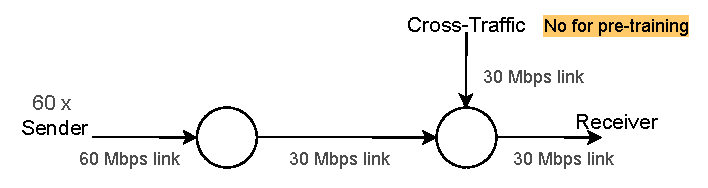
\includegraphics[scale=1.2]{figures/simple_topo.pdf}
    \caption{Initial topology for data generation}
    \label{fig:topo}
  \end{center}
\end{figure}

We begin with a simplified scenario of a single-link network topology which connects two hosts, via two switches as shown in Figure \ref{fig:topo}. For the pre-training dataset, each of $60$ senders generates $1Mbps$ of messages from the above mentioned distributions. They send messages over a bottleneck link with $30Mbps$ bandwidth and a queue size of $1000$ packets. We run $10$ simulations for $60$ seconds, each with randomized application start times in a $1-50$ second window. This also ensures none of the applications are too short to actually affect the overall dynamics of the network. The randomization of the start times ensures complex interactions between different flows, which lead to significant variation in dynamics of the network. This helps make the data for the pre-training capture a large, generic underlying distribution, which is hugely beneficial for fine-tuning on specific tasks later. This pre-training dataset contains about $1.2$ million packets. There is a possibility of introducing cross-traffic using a second source of disturbance on the second switch, however we turn it off for generating pre-training data, and try to learn general dynamics from a single bottleneck in the topology.

\begin{figure*}[h]
    \centering
    \begin{subfigure}[h]{0.5\textwidth}
        \centering
        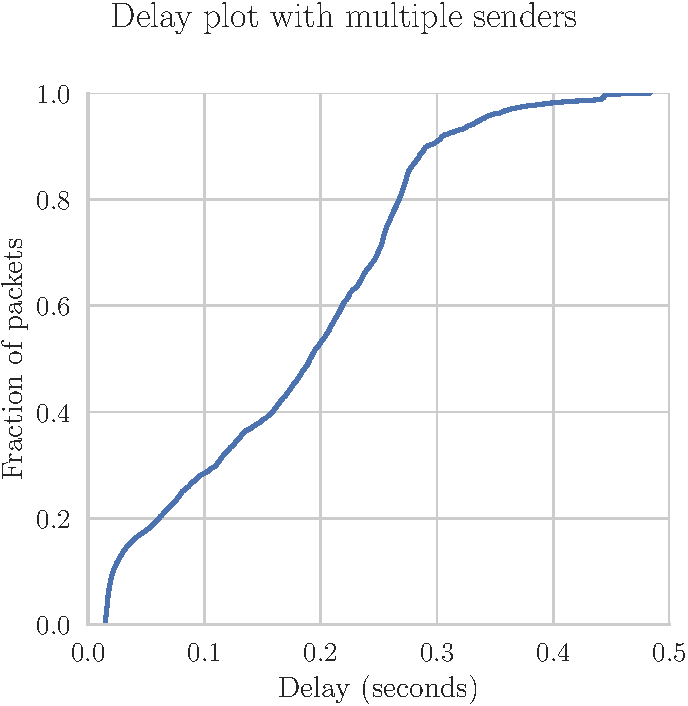
\includegraphics[scale=0.55]{figures/delay.pdf}
        \caption{Delay distribution, single run}
    \end{subfigure}%
    ~ 
    \begin{subfigure}[h]{0.5\textwidth}
        \centering
        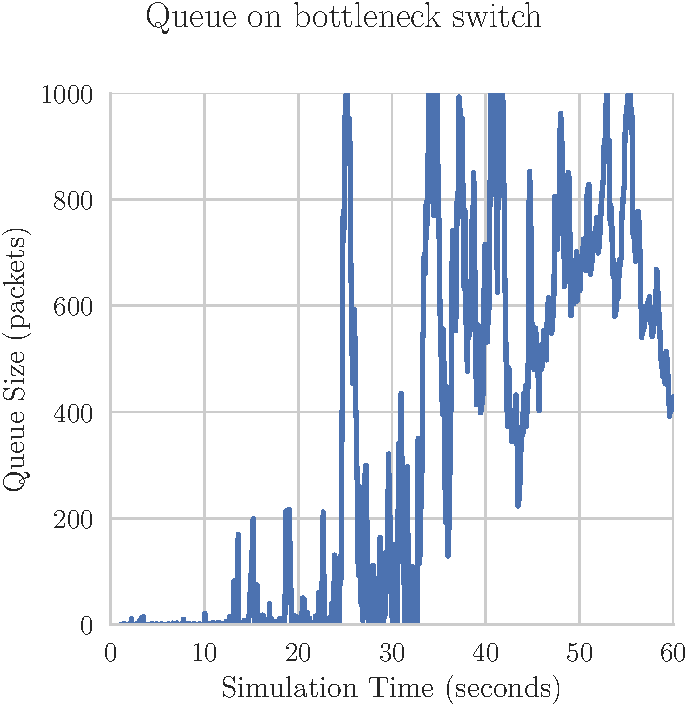
\includegraphics[scale=0.55]{figures/queue_profile_A.pdf}
        \caption{Queue profile on bottleneck queue}
    \end{subfigure}
    \caption{Distribution plots on pre-training data}
    \label{fig:datadist}
\end{figure*}

It is important to ensure that we do not have too much average behaviour in the generated data, else it will prevent the deep learning model from capturing the tail behaviour of the distributions. While in a lot of fields, learning average behaviour with deep learning is more or less enough, this idea fails with network data. In networks, worst-case scenarios can, even if occasionally, lead to significant network outages and data losses. In such an environment, it is crucial to understand the tail behaviour of the traffic distributions across various network applications, in order to truly learn the network characteristics and use the information gained to improve the performance of the network. We ensure that the features required for our training, end to end delay and packet size(we present the choice behind this selection in greater detail in Section \ref{ssec:desfeat}) have enough variation in our training data. We also ensure that the state of the queue on our bottleneck varies throughout the simulation, \ie it is neither always full and nor always empty, which introduces much more variation in the underlying dynamics of the training data. We refer to these distributions in Figure \ref{fig:datadist}


\section{Network Traffic Transformer (NTT)}
\label{sec:ntt}

We present our proof of concept Network Traffic Transformer (NTT~\ref{fig:ntt}) as a first Transformer model which is trained to learn sequence structure in network packet data and capture the underlying dynamics of the same, and generalize to new tasks based on the transfer learning principles from deep learning . However, learning the structure from network packet data can be extremely challenging. We face several major problems which need to be addressed.

\begin{enumerate}
\item \emph{Complexity of Data:} Network packet data is much more complex as compared to data from images(pixels) or from sentences(words). Packet data comes with several layers of hierarchy in terms of headers, protocol stack etc. We need to devise an effective way to choose features for learning, which captures all of the required information. At the same time, we need to ensure that we don't have redundancy in choosing the features,\ eg some fields across protocols and headers may present the same information in multiple ways. Choosing the features from packets which are the best learning becomes an incredibly hard task.

\item \emph{Time-Series Data:} Neither data in CV nor NLP follows a time series structure, but in network packet data it does, which poses a big challenge. The fate of a packet in the the data depends often on a packet much further in the past, which leads to the need to learn from extremely long sequences of data. As discussed, Transformers scale quadratically with in increasing sequence size, hence learning from long sequences is a challenge. At the same time, the fate of a packet may be affected much more by the more recent packets, which leads to the challenge of effectively learning from both short term and long term dynamics.

\item \emph{Training tasks:} The structure of data in NLP and CV is well understood by humans and it makes it easier to design pre-training and fine-tuning training objectives for these problems. Network packet data is extremely abstract and it significantly harder for us to parse this information and understand it. This makes developing such training objectives on network packet data a bigger challenge. We need to effectively design these in order that the sequence structure can be learnt to the best extent and in the most efficient manner possible.

\end{enumerate}

\begin{figure}[h]
  \begin{center}
    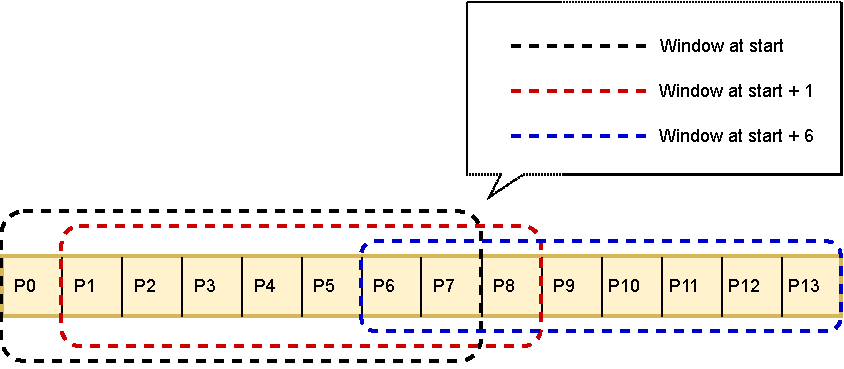
\includegraphics[scale=1]{figures/slidingwindow.pdf}
    \caption{Sliding window for sequence selection}
    \label{fig:sliding}
  \end{center}
\end{figure}


\subsection{Sequence definition}
\label{ssec:desseq}
An initial challenge which came up in our sequence modelling problem was choosing an appropriate sequence definition for our training and evaluation samples. In using Transformers for NLP, the concept of sequence is well defined in terms of either sentences or paragraphs, which come from the structure of most languages itself\footnote{We talk about structure in Indo-European languages here which is not universally true for all language families}. In using Transformers for CV, concept of sequence was artificially constructed using the concept of splitting the image into fixed size patches, which has been covered in detail in Section \ref{ssec:bgvit}. In our case, we have as pre-training data, a time-series dataset, in increasing order of timestamp from the first packet in the network trace.

As our network packet data sequence does not have natural delimiters, we introduce a concept of a sliding window over our packets, in order to create a fixed sequence length, which will then we provided as input to our NTT. We choose a \emph{one-step} sliding window of $1024$ packets as our sequence, which roughly matches the size of the queue on the bottleneck switch. At every step, we shift the sliding window forward by a single step and we illustrate this in Figure \ref{fig:sliding}. We expect that this will capture network behaviour when the queue is full and we hypothesise such a condition to be important for learning the dynamics. The concept of sliding windows has also been successfully used in cases on NLP data, which doesn't have the necessary delimiters in the data itself\cite{beltagyLongformerLongDocumentTransformer2020}, which makes such a design choice a natural starting point in our case. Our sliding window becomes a sequence of elements, which each individual element containing a certain number of features which are required for learning on our training objective.

Our pre-training data contains traces from multiple runs of simulation, in order to increase the richness of our pre-training data and enable us to learn variation in dynamics and generalise to a wide variety of tasks. These simulations represent network measurements taken at different points of time and it is important that our sliding windows always contain elements from the same run of simulation. Since data from different simulation represents independent measurements, we ensure that we construct our sliding windows independently over each run of the simulation data, and then use the data from the combination of these sliding windows as our training samples.

\begin{figure}[!hbt]
  \begin{center}
    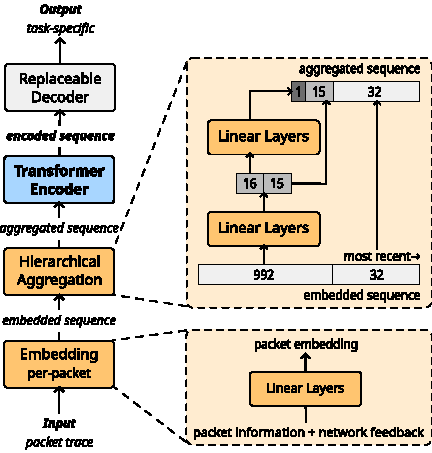
\includegraphics[scale=1.5]{figures/architecture_ntt.pdf}
    \caption{The Network Traffic Transformer (NTT) contains three main stages:  %
        an embedding layer, % for feature extraction,
        an aggregation layer, and
        a transformer encoder.
        It outputs a context-rich encoded sequence that is fed into a task-specific decoder.
        %
        The aggregation layer aggregates 1024 packet embeddings into 48 in two stages.
        The most recent packets are kept as-is, less recent packets are aggregated once, and the least recent twice.
    Credits: Alex, HotNets '22}
    \label{fig:ntt}
  \end{center}
\end{figure}

\subsection{Feature selection for the NTT}
\label{ssec:desfeat}

Packets carry a lot of information that could be used as model features, \eg all header fields, payload size etc. Today, we typically use networking domain knowledge to manually extract and aggregate features, then feed them into off-the-shelf standard ML architectures. This is done repeatedly for every task required, we always choose features which will be the best choice for learning our task objective and then, train a new ML model from scratch for every application.
We argue this is sub-optimal for two reasons:
\begin{itemize}
\item First, we always tailor these features to a specific task and dataset, which limits generalization. This process is redundant and never lets us benefit from previous training experiences and results.
\item Second, since the features are not learned from data, they may end up sub-optimal for the task. Choosing the right features for training an ML model is incredibly hard. The only foolproof method is to perform an exhaustive search over all possible combinations of features, and then choose the best performing set/subset of features. Several methods which do this are GridSearchCV and KFoldCV\cite{scikit-learn} but these methods are extremely slow and resource intensive.
\end{itemize}

We propose to let the model learn useful features from raw data. To learn traffic dynamics from a sequence of packets, we must provide the model with information about the packets as well as their fate in the network. Since we do not want to define a priori how important the individual pieces of information are, we feed them all into a first embedding layer~(\ref{fig:ntt}). The layer is applied to every packet separately. The embedding layer itself is a linear projection layer, which helps increase the representation of the information present in the selected features. Also, as these embeddings are learnable parameters in our NTT, over the training process, the model can learn which is the best representation for our input features, from the point of view of feeding information into the transformer encoder.

We argue that we need both information about the packet state and the network state to capture the overall network dynamics. In our proof-of-concept NTT, we use minimal packet and network
information and argue that the selected features have enough information to model the network dynamics which is needed for our training objectives.
\begin{itemize}
\item \emph{relative timestamp:} Transformer architectures process items in a sequence in parallel, hence they need some positional information in the input in order to understand the relative order of the elements in the sequence. These positional embeddings can be provided as fixed absolute\cite{vaswaniAttentionAllYou2017} or relative\cite{shaw2018selfattention} or as learned positional embeddings\cite{gehring2017convolutional}. Since our packet data is a time-series sequence, we use the relative timestamp to our first packet as a direct feature for our positional encoding information. The relative timestamp is part of the features passed through the embedding layer, and thus becomes a learnable value for a positional encoding.
\item \emph{packet size: } The packet size is used as a feature as it determines the fate of the packet from the packet state. The size of the packet affects the number of packets which can be accommodated in the queue buffer, \eg larger packets means less packets are present in the queue at the particular point in time. This helps in learning the dynamics of the fate of the packet which is directly affected by the state of other packets.
\item \emph{end-to-end delay: } The end to end delay in our setup includes both the queueing delay of the packet, along with the path delay. This delay reflects the state of the network at any given point of time, as the delay is caused by the complex interaction between packets and also reflects effects of tangible networks conditions such as congestion, packet drops etc.
\end{itemize}
These enable learning embeddings with temporal(evolution of delays over time) and spatial(impact of packet size on the delay) patterns.We discuss the challenge of embedding more information in future section.


\subsection{Learning packet aggregation}
\label{ssec:desagg}


CHANGES: A lot, right now the same as the HotNets paper

Packet sequences must be sufficiently long to capture more than short-term effects in traffic dynamics.
But as the training time of Transformers scales quadratically with the sequence length, we face practical limitations.
%to sequences tens-of-packets long.
% \alex{I have discussed this quickly with Siddhant. Transformers handle a few hundreds of inputs (e.g. BERT 512, ViT 256). We could also train with a sequence of about 600 packets, so there was no Transformer limitation. But: with the GPUs we have available, we are limited by memory -- if the sequences are too long, we cannot fit enough of them into memory at the same time, which slows down training a lot. So we train with 48, but the quadratic scaling is not the main bottleneck at this size.}

We address this problem by using multi-timescale aggregation~(\ref{fig:ntt}).
We aggregate a long packet sequence into a shorter one while letting the model learn how to aggregate the relevant historical information.%
%
\footnote{This is similar to the pixel patch aggregation in ViT~\cite{dosovitskiyImageWorth16x162021}.}
% Similar to transformers in CV which aggregate pixels in patches to scale, we need to aggregate packets to support packet sequences of more than tens of packets.
%
However, we aim to both aggregate \emph{and} retain recent packet-level details.
To achieve this, we keep the most recent packets without aggregation and the longer traffic is in the past, the more we aggregate, as packet-level details become less relevant to predict the current traffic dynamics.
%~(\cref{fig:aggregation}).
% However, a fixed aggregation size would mean giving up packet-level details.
% We leverage the time-series nature of traffic to get the best of both worlds.

In our proof-of-concept, we set the initial sequence length to 1024, matching roughly the number of in-flight packets in our experiments, which we aggregate into 48 elements. The right-hand side of \ref{fig:ntt} shows the aggregation details.
% Notably, we only pick rough `bin sizes' while the model learns how to perform the aggregation. 
Our multi-timescale aggregation is easy to adapt to a larger history without sacrificing recent packet details.
We show in eval that this aggregation is beneficial, but it is unclear which levels of aggregation generalize best; we discuss this further in future.
%We discuss this idea question further in~\cref{sec:future}.


\subsection{Learning network patterns}
\label{ssec:despatt}
% ========================================

Finally, we need a training task that allows NTT to learn network dynamics: in our proof-of-concept, we use end-to-end delay prediction.
We aim to get the pre-trained NTT to generalize well for a large set of fine-tuning tasks.
Consequently, we need a pre-training task that is generic enough to be affected by many network effects.
%Only then does learning the task lead to learning the dynamics.
As almost everything in a network affects packet delays (\eg path length, buffer sizes, etc.), a delay prediction task seems a rational choice.
%learning to predict them appears appropriate.

To pre-train NTT, we mask the delay of the most recent packet in the sequence and use a decoder with simple linear layers to predict the actual delay.
During training, the NTT must learn which features are useful (embedding layer), how to aggregate them over time (aggregation layer), and how the aggregated elements influence each other (transformer encoder layers).

During fine-tuning, one can replace the decoder~(\ref{fig:ntt}) to adapt NTT to a new environment (\eg a different network) or to new tasks (\eg predicting message completion times).
%new task---\eg predicting message completion times---or networking context---\eg in another network.
This is efficient as the knowledge accumulated by NTT during pre-training generalizes well to the new task, as we demonstrate in the next section.











